\documentclass[a4paper]{article}

\usepackage{fullpage} % Package to use full page
\usepackage{parskip} % Package to tweak paragraph skipping
\usepackage{tikz} % Package for drawing
\usepackage{amsmath}
%\usepackage{mathaccent}
\usepackage{hyperref}
\usepackage{subfigure}
\usepackage[utf8]{inputenc}
\usepackage[cyr]{aeguill}
\usepackage[frenchb]{babel}
\usepackage{graphicx}
\usepackage[]{algorithm2e}
\usepackage{xcolor}
\usepackage[]{float}
\usepackage{tikz}
\title{Compte Rendu - TP ETI5-IMI \\ \textit{Shaders avancés et Marching Cubes}}
\author{Di Folco Maxime - Girot Charly}
\date{27/10/2017}


\tikzset{my arrow/.style={
  blue!60!black,
  -latex
  }
  }
  

\begin{document}
\maketitle

%% Explication des noramles, Relecture partie 1 (à completer)
%% Toutes les images d'amelirotaion graphique des textures

\section{Parallax Mapping - Donner l'illusion du relief}
\subsection{Utilisation des textures de normales}
\textbf{Avant} : utilisation de textures \textit{colorées} appliquées directement sur un maillage. Exemple : dessiner un mur de briques comme sur la Fig.\ref{briques}

\begin{figure}[H]
\centering
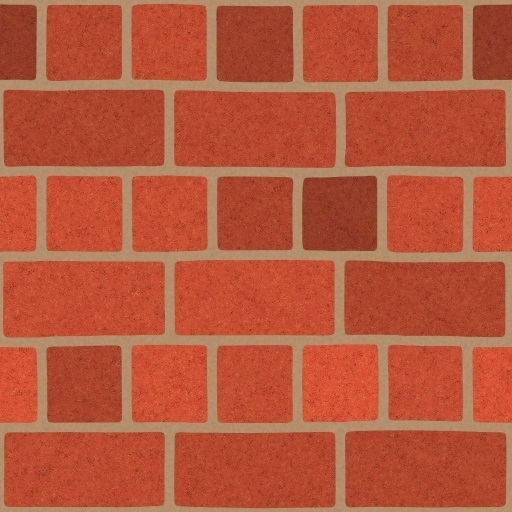
\includegraphics[width=0.3\textwidth]{figures/brick_diffuse.png}\label{briques}
\caption{Images à reconstruire sous la forme d'un panorama}
\end{figure}


\textbf{Désormais} : utilisation des textures pour d'autres informations et utilisations (modifications de normales Fig\ref{normales}, stockage d'informations de profondeurs Fig\ref{profondeur}). 

\begin{figure}[H]
\centering
\subfigure[]{\label{normales} 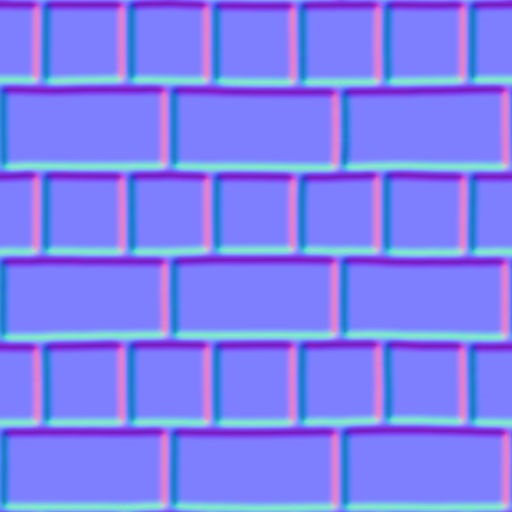
\includegraphics[width=0.3\textwidth]{figures/brick_normales.png}}
\subfigure[]{\label{profondeur} 
\includegraphics[width=0.3\textwidth]{figures/brick_profondeur.png}}
\caption{Textures contenant les informations de normales (a) et de profondeur (b)}
\end{figure}


Dans un premier temps, on nous fourni un programme qui implémente le normal mapping. On peut remarquer que la lumière est fixe mais les ombres évoluent en fonction de la rotation de l'objet. Il est possible de distinguer un relief entre les briques et leur support (le mur). Cela provient du fait que dans la méthode normal mapping les normales ne sont plus seulement orientés vers nous selon l'axe $z$ mais sont désormais liées aux axes $x$,$y$ et $z$ de la surface en fonction de la carte des normales representée Fig\ref{normales} où la composante rouge indique une modification de la normale selon l'axe $x$, verte pour l'axe $y$ et bleue pour l'axe $z$. Les normales ne sont ainsi plus toutes orientées dans le même sens selon la surface de l'objet, mais orientées différemment selon chaque fragment constituant notre objet. On obtient ainsi grâce à l'illumination des surfaces beaucoup plus détaillés.

\begin{figure}[H]
\centering
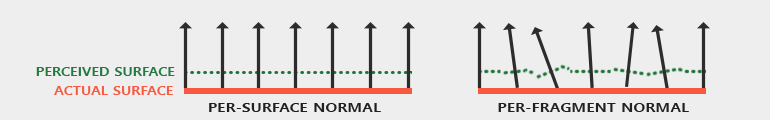
\includegraphics[width=0.5\textwidth]{figures/normalsOrientation.png}\label{normalOrientation}
\caption{Principe de l'orientation des normales en parallax mapping - tiré de :  https://learnopengl.com/\#!Advanced-Lighting/Normal-Mapping}
\end{figure}



Dans cette méthode, les tangeantes bi-tangeantes sont calculées dans l'espace TBN (Tangeante, Bitangeante, Normal). Dans cet espace les normales pointent toujours approximativement vers la direction z positive. La direction initiale est alors indépendante de l'orientation du plan initial. Après avoir appliqué une transformation sur notre plan, nous pouvons en utilisant une matrice spécifique transformer les vecteurs normaux initiales en les orientant le long de la direction de la surface cartographiée finale grâce à l'indépendance de la direction initiale par rapport à l'orientation du plan initial.

Pour simplifier nous aurions pu utiliser un simple normal mapping en orientant simplement la texture des normales selon la map. Les normales pointeraient alors vers en direction du plan normal du plan. Néanmoins, cela pose le problème suivant : il faut que les vecteurs normaux (qui pointent tous dans la même direction) et que la surface normale du plan auquel on applique la texture pointent dans la même direction pour obtenir un effet d'éclairage réaliste. Lorsque nous effectuons une transformation sur la position du plan normal, les vecteurs normaux ont été calculée selon une direction (celle de la map initiale) et donc pointeront toujours dans la même direction et pas en fonction de l'orientation du plan normal de la map transformée . L'éclairage n'aura donc pas l'air juste comme le montre la Fig \ref{lighting_problem}


\begin{figure}[H]
\centering
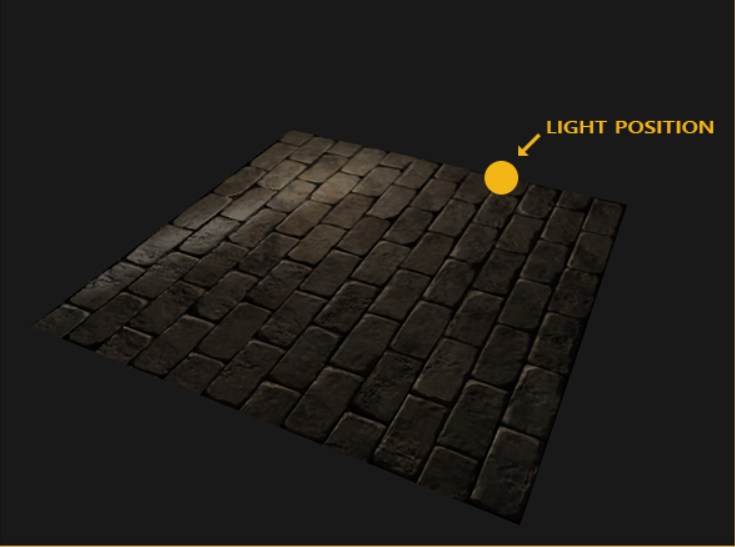
\includegraphics[width=0.5\textwidth]{figures/lighting_problem.PNG}\label{lighting_problem}
\caption{•}
\end{figure}

Dans ce programme, nous souhaitons pouvoir utiliser plusieurs texture avec d'autres informations d'utilisations comme la modification des normales et le stockage d'informations de profondeurs. Chaque texture sera stockée dans un indice GLTEXTUREn. En lisant le buffer courant activée et en sélectionnant la texture grâce à glActiveTexture(GLTEXTUREn)   nous pouvons relier la cible à la texture à l'aide glbindtexture(). Cela nous permet donc de pouvoir "jongler" entre les différentes structures. La fonction glActiveTexture(GLTEXTUREn) sélectionne la texture que les appels suivants affecteront jusqu'à l'activation d'une autre texture.

Q3\\  
Rôle de chaque variable dans les shaders Vertex Shader : \\
- in vec3 position; Sommet habituels \\
- in vec3 normal; Normal données \\
- in vec2 $tex_coords$; Coordonées de texture \\
- in vec3 tangent; in vec3 bitangent; Tangeante et bitangeante - - calculés précédemment 
 \\

On calcule la matrice TBN avec les lignes de codes suivantes :\\ 
out vec3 $vf\_frag\_pos$ = model * position ;\\
out vec2 $vf\_tex_coords$;\\
out vec3 $vf\_tangent\_light\_pos$ = TBN * $light\_pos$;\\
out vec3 $vf\_tangent\_view\_pos$ = TBN * $view\_pos$;\\
out vec3 $vf\_tangent\_frag\_pos$ = TBN * $vf\_frag_pos$;\\

Fragment Shader : en fonction de la direction de la lumière, de la vue et des fragments tangeants on peut calculer les directions de la vue et de la lumière 
En fonction des différentes textures envoyées (couleur (diffuse) et normales) et des coordonnées de texture, on peut calculer la couleur des fragments.
Les variables vf sont exprimées dans l'espace TBN (donc liées à la surface de l'objet). 
On utilise pas height tex car on fait du normal mapping pas du parallax mapping (pas encore).

\begin{figure}[H]
\centering
\subfigure[]{\label{noNormalesResult} 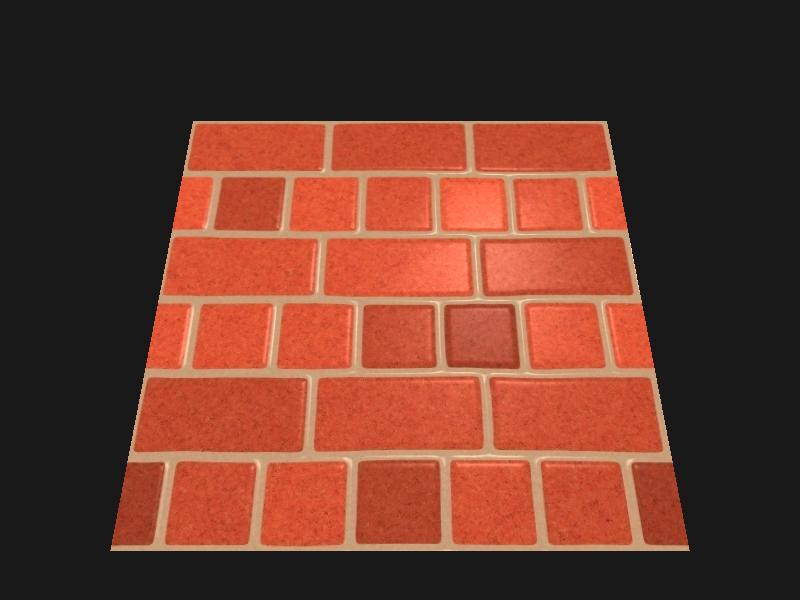
\includegraphics[width=0.3\textwidth]{figures/noNormalMapping.png}}
\subfigure[]{\label{NormalesResult} 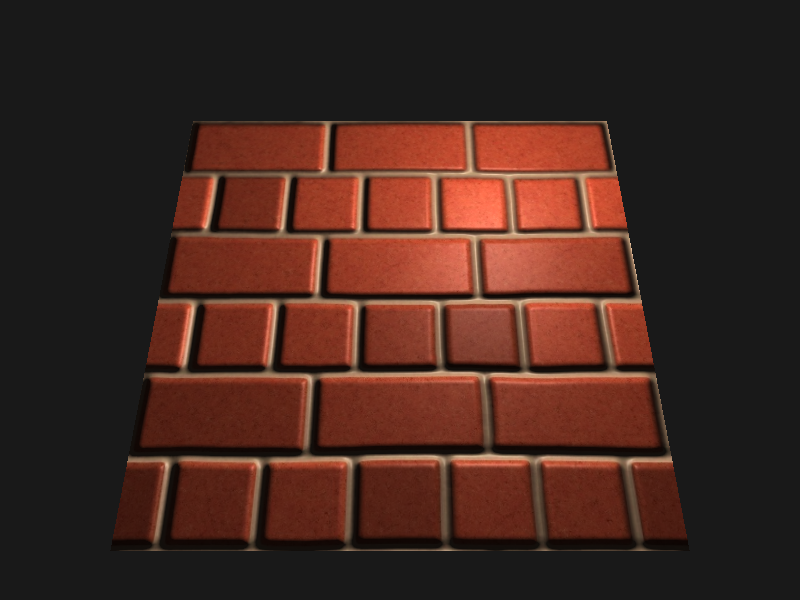
\includegraphics[width=0.3\textwidth]{figures/normalMapping.png}}
\caption{Résultat de l'application de texture couleur (a) auquel on applique la gestion des normales (b)}
\end{figure}


\subsection{Ajout d'un effet de profondeur avec l'utilisation des cartes de hauteur}
Modification des coordonnées de texture en fonction de la carte d'élévation et de la position de la vue. Explication géométrique de ce qu'on fait pour que donner cet effet de profondeur et du pourquoi ça marche mieux quand on a une vue rasante. 

On applique ensuite l'algorithme suivant pour ajouter l'effet de profondeur : 


\begin{figure}[H]
\centering
\subfigure[]{\label{normalResult} 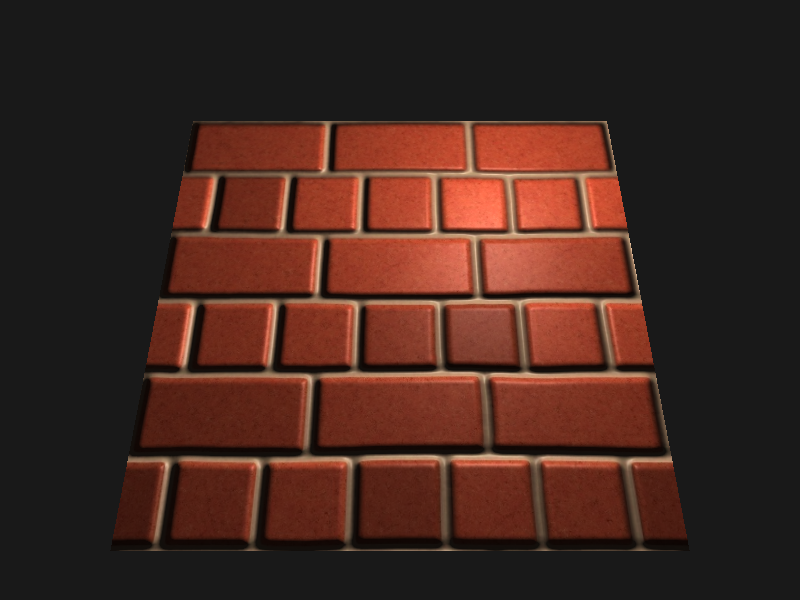
\includegraphics[width=0.3\textwidth]{figures/normalMapping.png}}
\subfigure[]{\label{ParallaxResult} 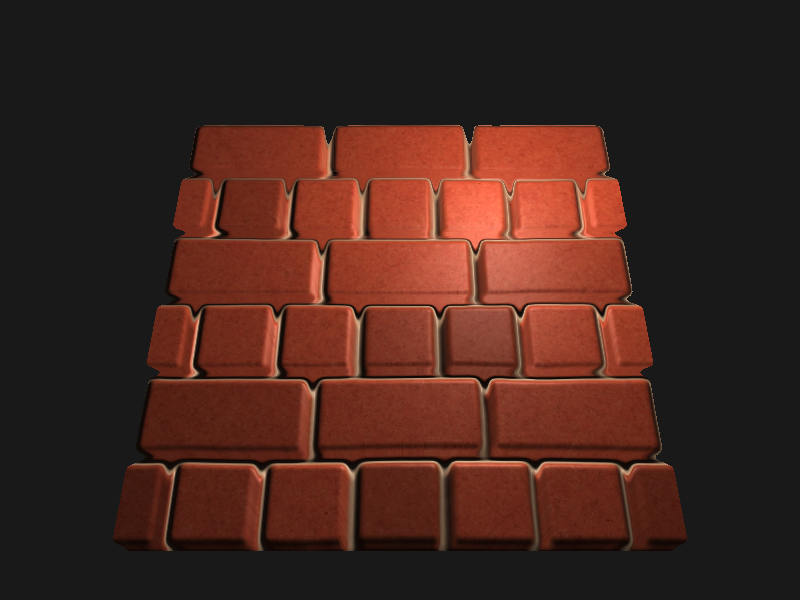
\includegraphics[width=0.3\textwidth]{figures/parallax1.png}}
\caption{Comparaison de la gestion des normales (a) auquel on applique une carte de hauteur (b)}
\end{figure}


Critique des limitations du parallax mapping.
\begin{figure}[H]
\centering
\subfigure[]{\label{normalResult} 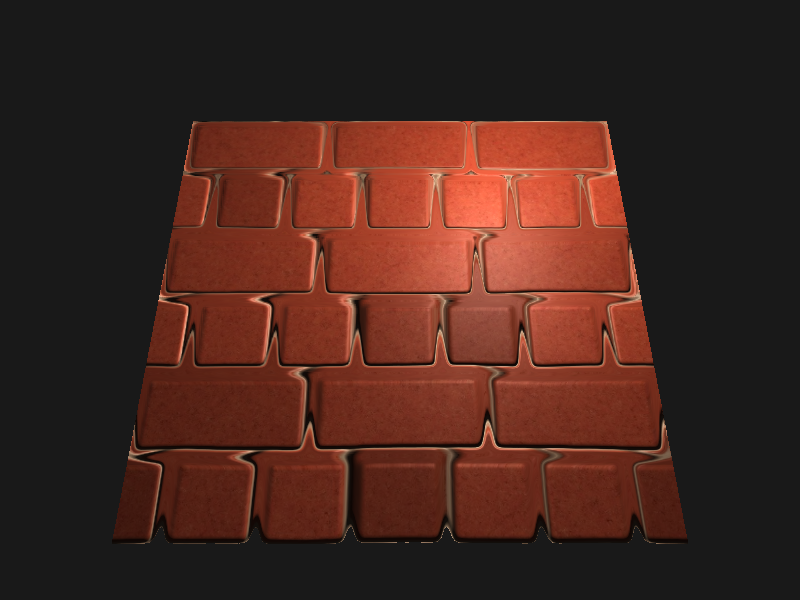
\includegraphics[width=0.3\textwidth]{figures/parallax2.png}}
\subfigure[]{\label{ParallaxResult} 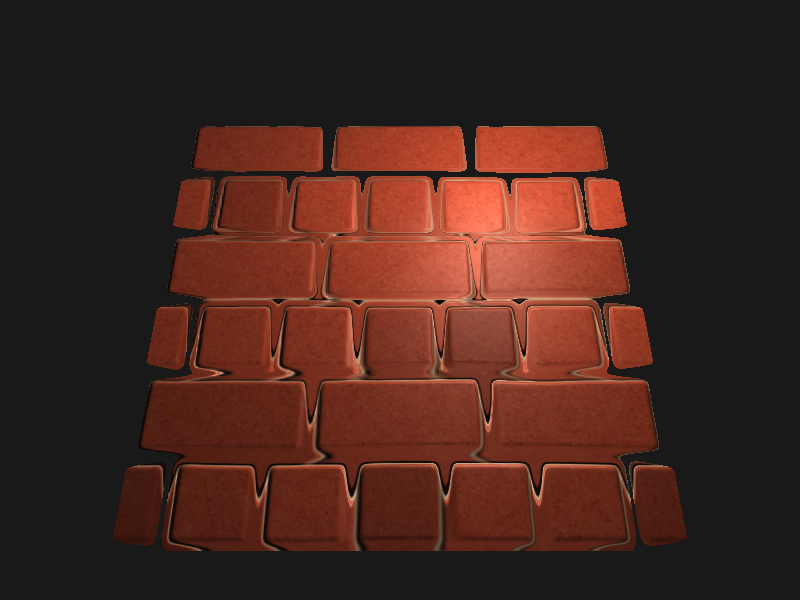
\includegraphics[width=0.3\textwidth]{figures/parallax3.png}}
\caption{Résultats de la carte des profondeurs pour un facteur de hauteur trop faible (a) trop haut (b)}
\end{figure}


\section{Marching Cubes}

%% En vrai je sais pas si faut vraiment répondre aux question une par une, c'est trop bizarre et j'ai même pas l'impression qu'il y ait de lien entre les questions ... 
\subsection{Présentation Générale}

Une surface pourrait être décrite par une fonction densité qui à chaque point 3D associe une valeur de densité. Une valeur positive de densité correspondrait à un point de la surface solide et une valeur négative à un espace vide. Grâce au GPU, nous allons générer des "blocs" de terrain, et les subdiviser en sous-blocs de 32x32x32 appelés voxels. Chaque sommet de ce sous-bloc possède une valeur de densité. L'algorithme de marching cubes nous permet de générer les polygones corrects dans chaque voxels en fonction de la valeur de densité de chaque coin.

%% PEut etre mettre une figure qui illustre ca 

Question 5 : Repérez quel groupe de shaders et quelle partie du code C++ sont liés à chaque étape. Essayez de faire un
schéma indiquant comment les différentes étapes echangent des données via des FBO ou des TF.

\begin{center}
\begin{tikzpicture}


\draw[step=0.5cm,white,very thin] (-6,-5) grid (6,10) ;
\fill[blue!40!white] (-2,10) rectangle (2,9);
\node[above] at (0,9.25){Build Density Verrtex};



\fill[blue!40!white] (-2,8.5) rectangle (2,7.5) ;
\node[above] at (0,7.75){Build Density Geometry };

\fill[blue!40!white] (-2,7) rectangle (2,6);
\node[above] at (0,6.25){Build Density Fragment };


\fill[blue!40!white] (-2,5.5) rectangle (2,4.5);
\node[above] at (0,4.75){List triangle vertex };

\fill[blue!40!white] (-2,4) rectangle (2,3);
\node[above] at (0,3.25){List Triangle geom};

\fill[blue!40!white] (-2,2.5) rectangle (2,1.5);
\node[above] at (0,1.75){List Triangle fragment };

\fill[blue!40!white] (-2,1) rectangle (2,0);
\node[above] at (0,0.25){Generer Vertices Vertex };

\fill[blue!40!white] (-2,-0.5) rectangle (2,-1.5);
\node[above] at (0,-1.25){Generer Vertices Geom};

\fill[blue!40!white] (-2,-2) rectangle (2,-3);
\node[above] at (0,-2.75){Gen Vertices Fragment };

\fill[blue!40!white] (-2,-3.5) rectangle (2,-4.5);
\node[above] at (0,-4){Render Vertex  };
\node[above] at (0,-4.5){+ Render Fragment};


\node[above] at (0,-5){Ordre d'utilisation des shaders - Ajouter Fleches et explications };
\end{tikzpicture}
\end{center}


\subsection{Analyse Du code}
Question 6 : Lisez la documentation de la fonction glDrawArraysInstanced , que réalise cette fonction ? Aurait-on pu s’en
passer ? Quelle est l’utilisation plus classique de cette fonction ?

De la même manière que glDrawArrays permet de "dessiner/rendre" une primitive (un triangle dans notre cas), glDrawArraysInstances permet de synthétiser une série instanciée de primitives. On aurait donc pu s'en passer en utilisant glDrawArrays dans une boucle avec itération des indices de chaque primitive (ce qui est fait automatiquement avec cette fonction). 

Question 7 : Comment s’utilise la fonction glActiveTexture ? 


\subsection{Amélioration de l'algorithme}

Question 8 : Dans les shaders, on trouve des variables de type isampler2D et d’autres de type sampler2D. Quelle est la
différence entre ces deux types ?  Que réalise la fonction texelFetch ?

Les documentations font réferences à \textit{g}sampler2d ou g est remplacé par rien, u ou i. Rien signifie que le sampler2D contenant des coordonnées de textures sera exprimé en float, i par des entiers signés et u par des entiers non signés. 

TexelFetch recherche le texel (pixel de texture) correspondant à la coordonnées de texture qui lui a été fournit et à la texture. 

Question 9 : Corrigez le calcul des normales en supposant que sa direction est donnée par le gradient de la fonction de
densité. Quel fichier avez-vous modifié pour cela ?



L’aspect crénelé de la sphère vient du fait que la position des vertex est toujours choisie au milieu des arètes des cubes.
Une meilleure approche consiste à réaliser une interpolation linéraire pour choisir cette position.
Question 10 : Réalisez cette interpolation de manière à obtenir une sphère bien lisse comme celle de la figure 9.

\begin{figure}[H]
\centering
\subfigure[]{\label{mc0} 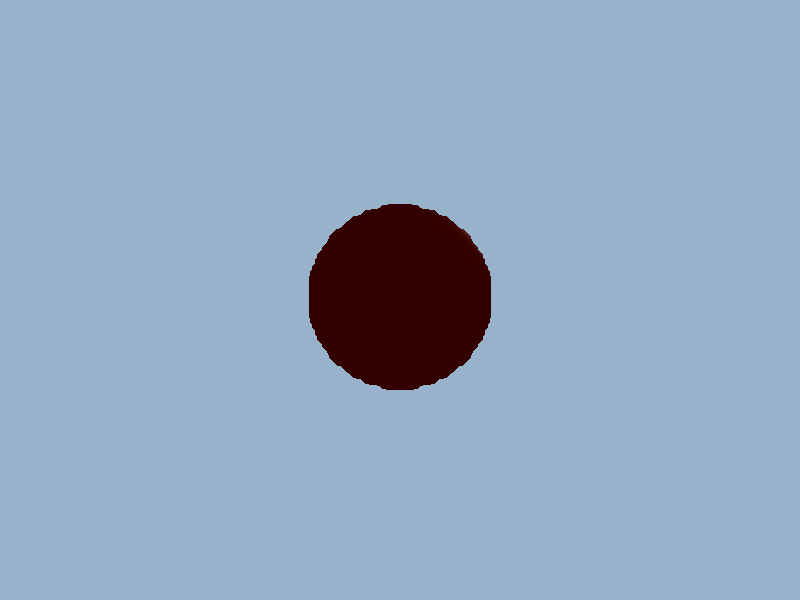
\includegraphics[width=0.3\textwidth]{figures/mc0.png}}
\subfigure[]{\label{mcNormalResult} 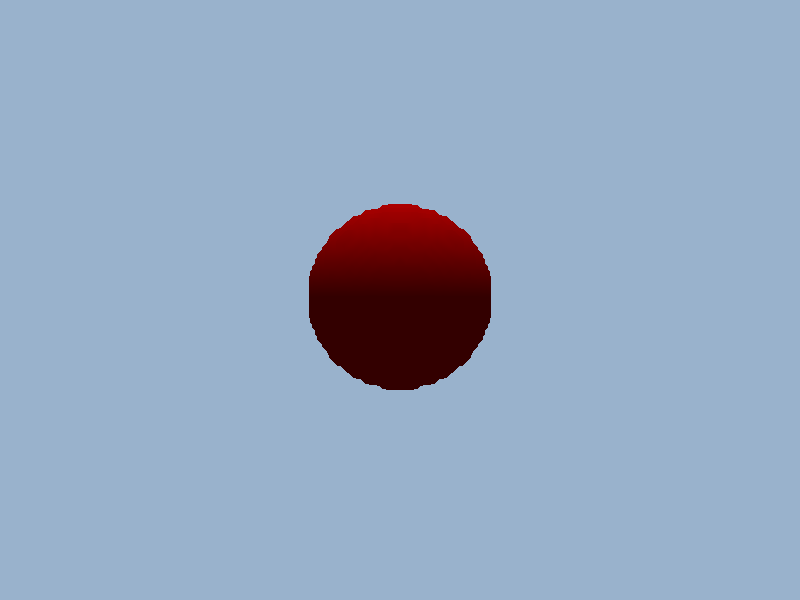
\includegraphics[width=0.3\textwidth]{figures/mcnorm.png}}
\subfigure[]{\label{mcInterResult} 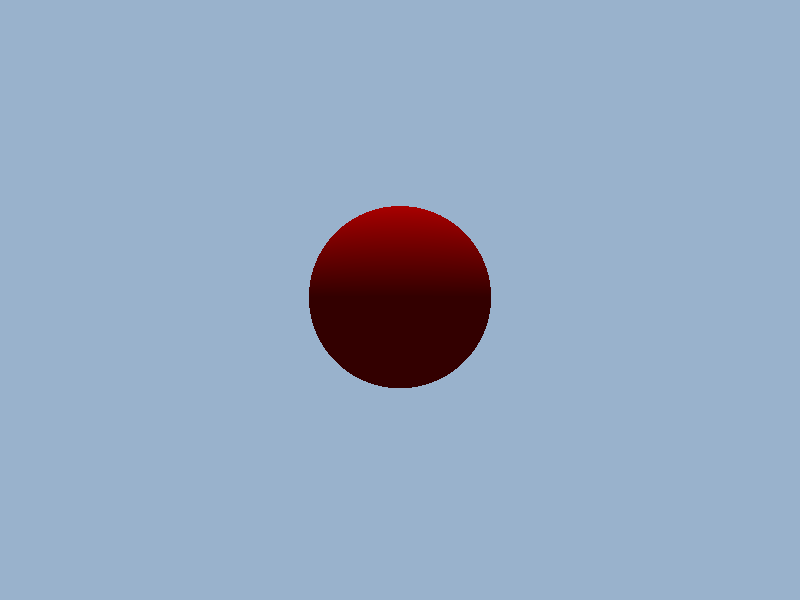
\includegraphics[width=0.3\textwidth]{figures/mcnorminterp.png}}
\caption{Marching Cubes Original (a) ; Calcul des normales fonction du gradient de la fonction de densité (b); Interpolation linéaire de placement des vertex par rapport aux arrètes (c)}
\end{figure}


\subsection{Fonction de densité}

Images des différentes fonctions de densité qu'on peut réaliser + celle de la plus intéressante qu'on ait 

\begin{figure}[H]
\centering
\subfigure[]{\label{mc0} 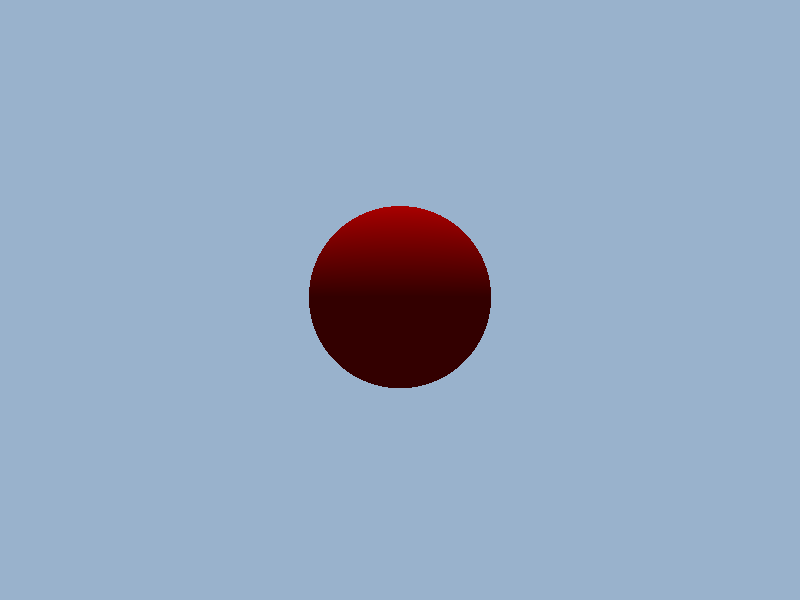
\includegraphics[width=0.3\textwidth]{figures/mcnorminterp.png}}
\subfigure[]{\label{mcNormalResult} 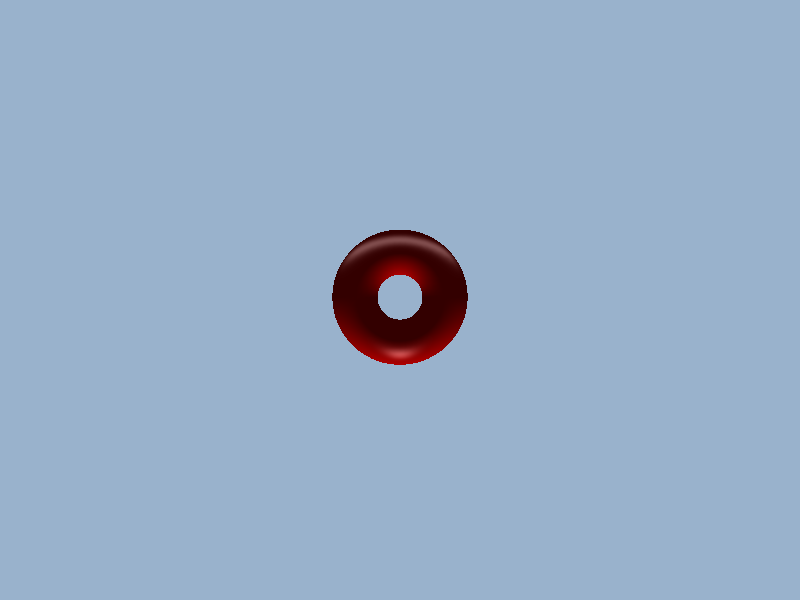
\includegraphics[width=0.3\textwidth]{figures/torus.png}}
\subfigure[]{\label{mcInterResult} 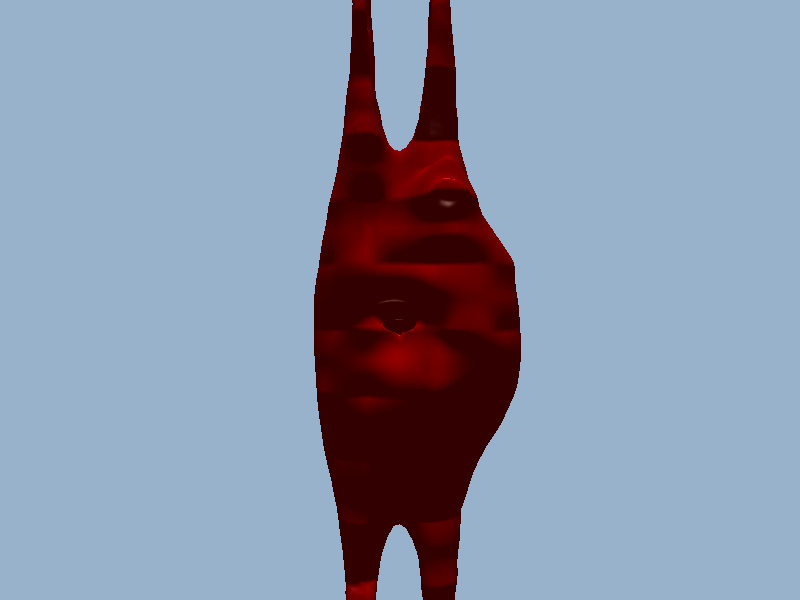
\includegraphics[width=0.3\textwidth]{figures/chelouA.png}}
\caption{Marching Cubes avec différentes fonctions de densite : Boule (a), Torus (b), Création de roches (c)}
\end{figure}

\subsection{Amélioration graphique \& Textures}


Question 12 : Mettez en place le calcul pondéré des textures par les normales pour obtenir une image du genre de la
figure 18.



\subsection{Combinaison Parallax Mapping + Marching Cubes}


\bibliographystyle{plain}
\bibliography{bibliography.bib}
\end{document}